\documentclass{mcgillhomework}

\titledeclaration{COMP 273 - Classical CPU Project}{Julian Lore}{260741656}{Sandrine Monfourny-Daigneault}{260692380}{Jacques Vincent}{260744151}{Joseph Vybihal}{April 10th 2017} % Change submission date as needed
\hdrdeclaration{Lore, Monfourny, Vincent}{COMP 273 - Classical CPU Project}
\title{A Comprehensive Guide to the OK-Computer}
\date{April $\text{10}^{\text{th}}$, 2017}
\author{Julian Lore (260741656)
\\ Sandrine Monfourny-Daigneault (260692380)
\\ Jacques Vincent (260744151)}
\usepackage{graphicx}
\usepackage{tabularx}
\begin{document}

%\createtitlepage
\maketitle
\begin{center}
		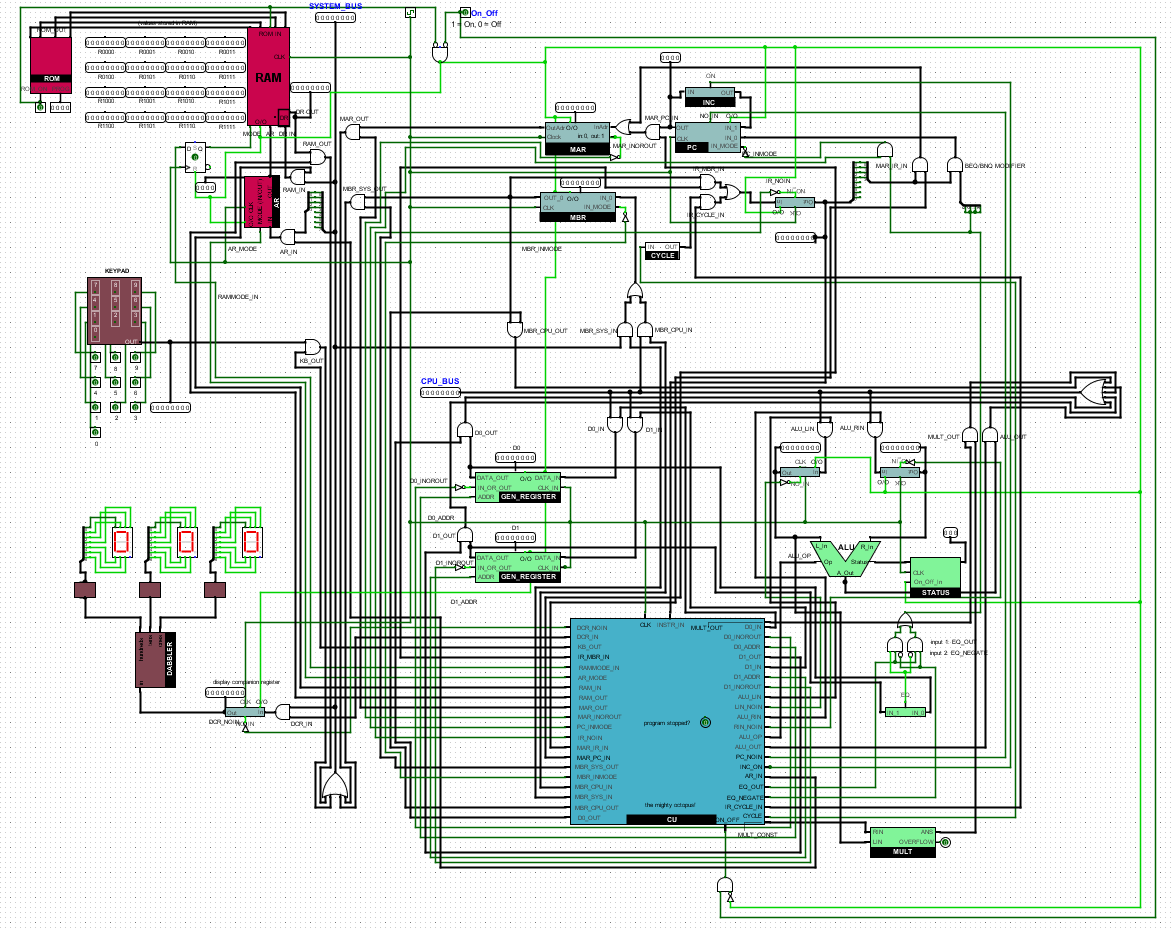
\includegraphics[scale=0.4]{CPU}
	\end{center}
		\tableofcontents
		\newpage
	\pagestyle{mainmatter}
	\pagenumbering{arabic}
	\markright{Lore, Monfourny-Daigneault, Vincent: The OK-Computer}
	\pagestyle{myheadings}
	\section{CPU Structure}
	\paragraph{Power}~
	\\ 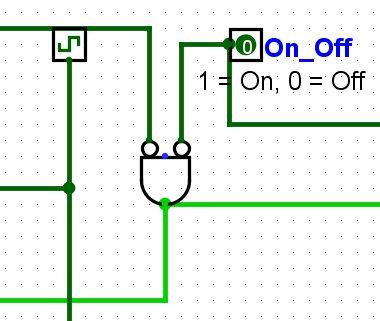
\includegraphics[scale=0.5]{ON}\\The on button allows the CU to operate and perform instructions. When it is off and the ROM is also off, all data of the CPU is reset.
	\paragraph{RAM}~
	\\ 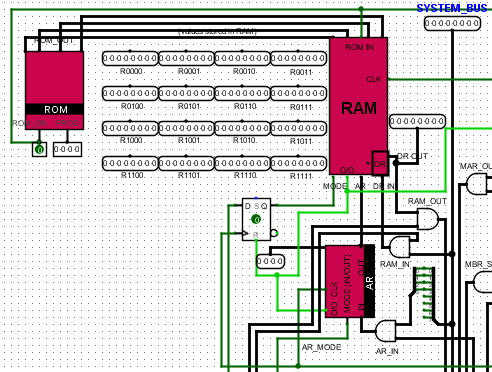
\includegraphics[scale=0.5]{RAM} \\The RAM is connected to the ROM and its $3$ respective registers, the mode, data and address registers. The ROM acts as an override to the usual ROM registers, OR gating the input of each byte in order to fill up all of RAM in one tick. The output pins next to the RAM indicate the values that all the bytes of RAM are storing. The mode register is controlled by the CU and the data and address register receive input from the bus, with the CU controlling the gates that let data through.
	\paragraph{MAR/MBR}~
	\\ 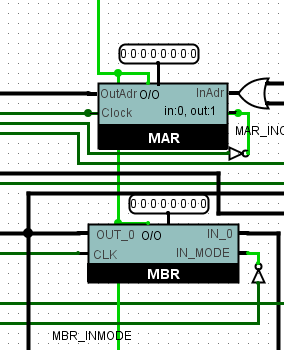
\includegraphics[scale=0.7]{MARMBR} \\The MAR and MBR have corresponding output pins displaying their contents. They have an in/out input that controls whether they are outputting data or inputting data. They output data by default in order to not intake 0s when nothing is specifically being sent to them. The MAR receives input either from the IR (for instruction arguments) or the PC (in order to load the corresponding address' instruction). The MBR receives input from either of the data registers, or from RAM through the bus.The MAR outputs to RAM's AR through the bus, while the MBR outputs to either the RAM's DR through the bus, any of the general registers or the IR.
	\paragraph{PC \& INC}~
	\\ 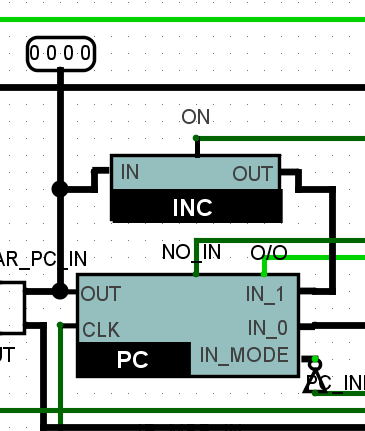
\includegraphics[scale=0.5]{PC} \\ The PC's incrementer increments whenever the CU reports that it is done an instruction and thus updates the PC's contents. The PC also receives an address from the IR if BEQ or BNEQ results in true. The PC also has an in/out mode.
	\paragraph{IR}~
	\\ 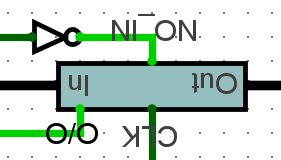
\includegraphics[scale=0.5]{IR} \\ The IR receives data from the MBR whenever the CU requests a new instruction. The IR delivers its op-code and operands to the CU for parsing.
	\paragraph{ALU}~
	\\ 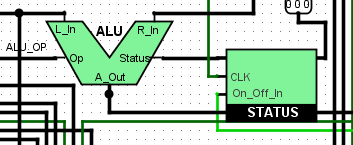
\includegraphics[scale=0.5]{ALU} \\ The ALU receives arguments from the general data registers and performs the operation specified by the op code given by the CU. It puts its answer in A Out which goes to the specified general purpose register and has a status register that will specify whether there were any errors with the operation.
	\paragraph{Mult \& EQ}~
	\\ 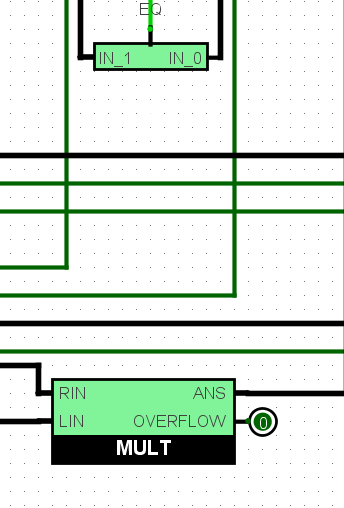
\includegraphics[scale=0.5]{MEQ}\\ The MULT and EQ circuits complement the ALU in order to parse the bonus MULT instruction and BEQ and BNEQ.
	\paragraph{General Purpose Registers}~
	\\ 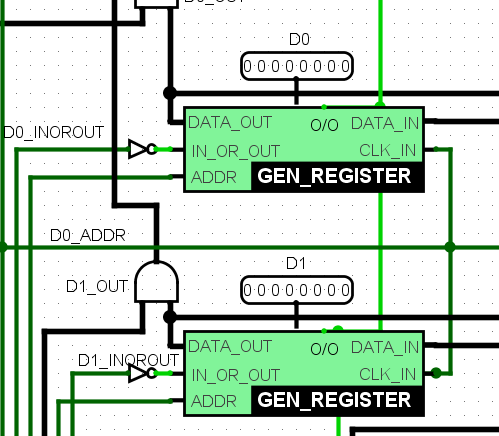
\includegraphics[scale=0.5]{DR}\\The General purpose registers receive input from either the MBR or the ALU. They have in or out modes and address inputs, which allows the CU to ask for either of the registers in particular.
	\paragraph{CU}~
	\\ 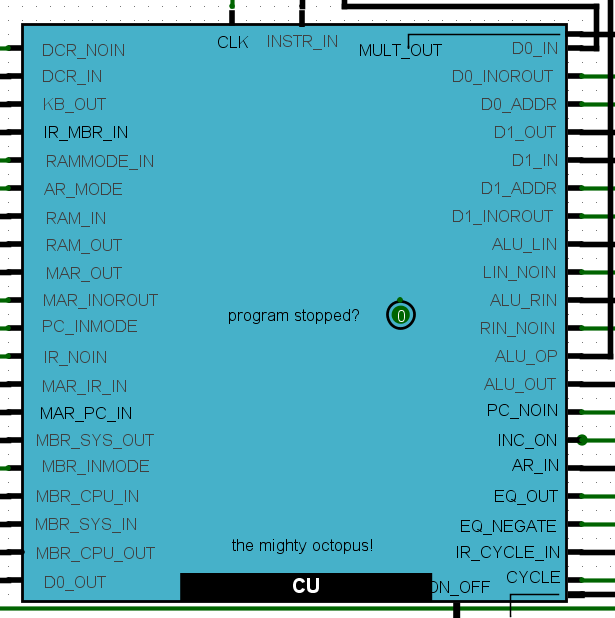
\includegraphics[scale=0.5]{CU}\\The CU receives an op code and operands from the IR and opens up the required gates for the instruction. It has a counter itself to go through the respective micro-instructions of each instruction. The CU is connected to almost every gate and input/output pins that control data flow.
	\paragraph{Display}~
	\\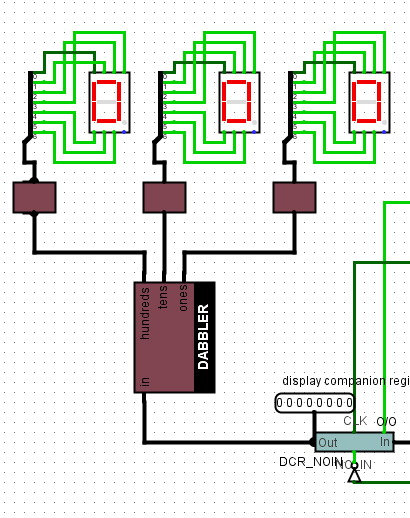
\includegraphics[scale=0.5]{DIS}\\The display has a companion register that receives input from the general purpose data registers through the bus and has its input controlled by the CU. The display uses the Double Dabble algorithm in order to convert a byte into BCD (Binary-coded decimal) in order to display a byte as $3$ decimal numbers. The corresponding BCD numbers are linked to 7-segment displays that map to the corresponding decimal numbers.
	\paragraph{Keypad}~
	\\ 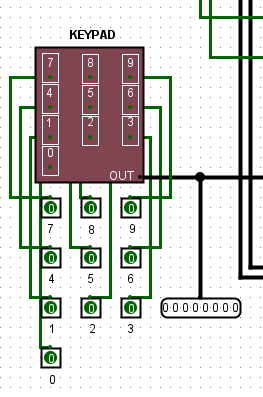
\includegraphics[scale=0.5]{KP}\\The keypad has a companion register that receives the button pressed as a binary number. The number is sent to a specified general purpose register through the bus and the MBR when requested by the CU.
	\section{Programs}
	For information on how to get programs running, read the included README.txt.
	\subsection{Required Program}
	What this program does:
	\\*  Multiplies (using adder in a loop) a number from RAM and a number from input buffer (keypad), answer displayed on display
	\\* Assume 1111 is the RAM value that stores the number we want to multiply by
	\\*
	\begin{tabular}{|c|c|l|}
		\hline \textbf{RAM Address} & \textbf{RAM contents} & \textbf{Description}
		\\* \hline 	0000	& 0111 1000 & \# Load input into D1
		\\* \hline 	0001	& 0101 0111 & \# If D0 isn't $0$, go to prog loop
		\\* \hline 	0010	& 1000 0000 & \# STOP, ends execution of program
		\\* \hline 	0011	& 0000 0000 & \# Will store counter the we'll increment
		\\* \hline 	0100	& 0000 0000 & \# Where we'll store answer
		\\* \hline 	0101	& 0000 0110 & \# Number we want to multiply by, 6 as example
		\\* \hline 	0110	& 0000 0001 & \# $1$ for incrementing
		\\ \hline
	\end{tabular}
	\\*
	\\* Prog:
	\\*
	\begin{tabular}{|c|c|l|}
		\hline \textbf{RAM Address} & \textbf{RAM contents} & \textbf{Description}
		\\* \hline 	0111	& 1010 0100 & \# Load current answer into D0
		\\* \hline 	1000	& 1011 0101 & \# Load number we want to multiply by into D1
		\\* \hline 	1001	& 0010 0000 & \# $D0=D0+D1$
		\\* \hline 	1010	& 0110 0000 & \# Prints current answer
		\\* \hline 	1011	& 1110 0100 & \# Store D0 into current answer
		\\* \hline 	1100	& 1010 0011 & \# Load counter into D0
		\\* \hline 	1101	& 1011 0110 & \# Load one into D1
		\\* \hline 	1110	& 0010 0000 & \# $D0=D0+D1$, increment counter
		\\* \hline 	1111	& 1110 0011 & \# Store D0 into counter
		\\ \hline
	\end{tabular}
	\\*
	\\* Rely on natural looping of CPU
	\\*
	\subsection{Modified Required Program}
	Does the exact same thing as the required program, but uses the bonus MULT instruction.
	\\\begin{tabular}{|c|c|l|}
		\hline \textbf{RAM Address} & \textbf{RAM contents} & \textbf{Description}
		\\ \hline 0000 & 0111 1000 & \# Load input into D1
		\\ \hline 0001 & 1001 1110 & \# $D1=D1\times constant(6)$
		\\ \hline 0010 & 0110 1000 & \# Print D1
		\\ \hline 0011 & 1000 0000 & \# Stop
		\\ \hline
	\end{tabular}
	\subsection{Countdown}
	Counts down from $255$ to $1$, showing the number on the display after every step.
	\\\begin{tabular}{|c|c|l|}
		\hline \textbf{RAM Address} & \textbf{RAM contents} & \textbf{Description}
		\\ \hline 0000 & 1010 1000& \# Load current number into D0
		\\ \hline 0001 & 0110 0000 & \# Print D0
		\\ \hline 0010 & 1011 1001 & \# Load $1$ into D1
		\\ \hline 0011 & 0100 0111 & \# BEQ, STOP if current number is $1$
		\\ \hline 0100 & 0011 0000 & \# $D0=D0-D1$
		\\ \hline 0101 & 1011 1010 & \# Load $0$ into D1
		\\ \hline 0110 & 0101 0001 & \# BNEQ, jump to beginning
		\\ \hline 0111 & 1000 0000 & \# STOP
		\\ \hline 1000 & 1111 1111 & \# Current number
		\\ \hline 1001 & 0000 0001 & \# One
		\\ \hline 1010 & 0000 0000 & \# Zero
		\\ \hline
	\end{tabular}
	\section{Description of Instructions}
	\begin{enumerate}
		\item (CYCLE)\\
		\begin{tabularx}{\textwidth}{|X|}
			\hline 000
			\\ \hline Op-Code
			\\ \hline 0-2
			\\ \hline
		\end{tabularx}
		Not a real instruction (in the sense that it isn't a part of any program), it's what the CU uses to prepare the next instruction in RAM
		
		\item LOAD: LD\\
		\begin{tabularx}{\textwidth}{|X|X|X|}
			\hline 101 & x & xxxx
			\\ \hline Op-Code & Register & Address
			\\ \hline 0-2 & 3 & 4-7
			\\ \hline
		\end{tabularx}
		Loads the contents at an address(4-7) of RAM into a selected data register(3). The address is sent to the MAR, which is then sent to the AR. The MODE is set to read mode and the contents located at the specified address are sent to the DR, then to the MBR. Then, the contents of the MBR are sent to the specified register.
		
		\item STORE: STR\\
		\begin{tabularx}{\textwidth}{|X|X|X|}
			\hline 111 & x & xxxx
			\\ \hline Op-Code & Register & Address
			\\ \hline 0-2 & 3 & 4-7
			\\ \hline
		\end{tabularx}
		Stores the contents of a selected data register(3) into an address(4-7) of RAM. The contents of the specified register are sent to the MBR. The address is sent to the MAR, which is then sent to the AR. The MODE is set to write mode and the contents of the MBR are sent to the DR, which then sends the contents to the byte of RAM at the specified address.
		
		\item ADD: ADD\\
		\begin{tabularx}{\textwidth}{|X|X|}
			\hline 0010 & x
			\\ \hline Op-Code & Register to store into
			\\ \hline 0-3 & 4
			\\ \hline
		\end{tabularx}
		Adds the $2$ data registers together and stores it into a register of choice (4). The contents of D0 are sent to the ALU through the bus. The contents of D1 are also sent to the ALU through the bus. For both of these, the CU activates the output mode on D0 and D1. Then, the ALU is set to add mode and the addition is done. Then, the result is sent to D0 through the bus and by activating the input mode on D0.
		
		\item SUBTRACT: SUB\\
		\begin{tabularx}{\textwidth}{|X|X|}
			\hline 0011 & x
			\\ \hline Op-Code & Register to store into
			\\ \hline 0-3 & 4
			\\ \hline
		\end{tabularx}
		SStores the result of subtracting the unspecified register from the specified register(4) into the specified register. Subtracts The contents of D0 are sent to the ALU through the bus. The contents of D1 are also sent to the ALU through the bus. For both of these, the CU activates the output mode on D0 and D1. Then, the ALU is set to subtract mode and the addition is done. Then, the result is sent to D0 through the bus and by activating the input mode on D0.  
		
		\item Branch equal: BEQ\\
		\begin{tabularx}{\textwidth}{|X|X|}
			\hline 0100 & x
			\\ \hline Op-Code & Address
			\\ \hline 0-3 & 4-7
			\\ \hline
		\end{tabularx}
		Checks whether both data registers are equal, if they are, jumps to the specified address (4-7). The contents of D0 and D1 are directly sent to a comparison checker. When they are equal, it outputs TRUE, and this output is sent to the PC. When/if it receives this TRUE signal, it will load the adress specified.
		
		\item Branc not equal: BNQ\\
		\begin{tabularx}{\textwidth}{|X|X|}
			\hline 0101 & x
			\\ \hline Op-Code & Address
			\\ \hline 0-3 & 4-7
			\\ \hline
		\end{tabularx}
		Checks whehter both data registers aren't equal, if they aren't jumps to specified address (4-7). The contents of D0 and D1 are directly sent to a comparison checker. When they are not equal, it outputs TRUE, and this output is sent to the PC. When/if it receives this TRUE signal, it will load the adress specified.
		
		\item PRINT: PRT\\
		\begin{tabularx}{\textwidth}{|X|X|}
			\hline 0110 & x
			\\ \hline Op-Code & Register to display
			\\ \hline 0-3 & 4
			\\ \hline
		\end{tabularx}
		Prints the decimal value of the specified data register (4) to the display. The contents of the specified register are sent to the MBR through the bus, which are then sent to the Display Companion Register through the bus. Then, the display will show whatever is stored in the register.
		
		\item INPUT: INP\\
		\begin{tabularx}{\textwidth}{|X|X|}
			\hline 0111 & x
			\\ \hline Op-Code & Register to store into
			\\ \hline 0-3 & 4
			\\ \hline
		\end{tabularx}
		Loads the value of the button pressed on the keyboard into the specified data register(4). The input is converted to binary and sent to the MBR through the bus, which is then sent to the specified register through the bus.
		
		\item STOP: STOP\\
		\begin{tabularx}{\textwidth}{|X|}
			\hline 1000
			\\ \hline Op-Code
			\\ \hline 0-3
			\\ \hline
		\end{tabularx}
		Permanently activates a pin in the CPU, which prevents the CYCLE command from being executed and therefore stops the program.
		
		\item MULTIPLICATION: MULT\\
		\begin{tabularx}{\textwidth}{|X|X|X|}
			\hline 1001 & x & xxx
			\\ \hline Op-Code & Register to store into & Constant
			\\ \hline 0-3 & 4 & 5-7
			\\ \hline
		\end{tabularx}
		Multiplies the specified data register (4) by a constant (5-7) and stores it in the original register. The contents of the specified register are sent to the left temporary register of the ALU. The instruction is sent to the CU, which isolates the constant stored within the instruction. Both of these are sent to the MULT calculator, which performs the operation and sends the output to the MBR, which then gets sent back to the specified register.
		
	\end{enumerate}

\end{document}